\section{SYSTEM MODEL AND PROBLEM FORMULATION}
\label{sec:prelim}
DA-HELLO acts on neighbour state that a node holds, so this section defines what a node can know and how that state reaches it. It introduces the two state carriers that organise the rest of the paper and contains no parameter values; those are given in Section~\ref{sec:eval}.

\subsection{Network and Mobility}
\label{sec:network}
A set of relays $\mathcal{S}=\{s_1,\dots,s_N\}$ and one fixed sink $s_0$ share an acoustic medium in a three-dimensional volume (Fig.~\ref{fig:network}). Each relay $s_i$ has a position $\mathbf{p}_i(t)$, a depth $z_i(t)$, a residual energy $e_i(t)$, a queue, learning variables, and timers. Sensing nodes generate packets, and every packet is addressed to the sink and relayed hop by hop.

Relays drift with the water. The velocity of relay $s_i$ follows a Gauss--Markov process with memory $\zeta$ around a position-dependent mean flow $\boldsymbol{\mu}(\mathbf{p})$,
\begin{equation}
\mathbf{v}_i(t{+}\Delta)=\zeta\,\mathbf{v}_i(t)+(1-\zeta)\,\boldsymbol{\mu}(\mathbf{p}_i)+\sqrt{1-\zeta^2}\,\boldsymbol{\Sigma}\,\mathbf{w}_i,
\label{eq:gm}
\end{equation}
where $\mathbf{w}_i$ is standard Gaussian noise and $\boldsymbol{\Sigma}$ sets the per-axis deviation. The mean flow models a mesoscale eddy as a counter-clockwise tangential flow around a centre $\mathbf{c}$ with radius $R$ and peak speed $V$,
\begin{equation}
\boldsymbol{\mu}(\mathbf{p})=V\,\min\!\Big(\tfrac{\rho}{R},1\Big)\,\hat{\mathbf{e}}_\theta,\qquad \rho=\|\mathbf{p}_{xy}-\mathbf{c}\|,
\label{eq:eddy}
\end{equation}
so nodes at different radii move differently and links break and form. The sink is stationary. A relay that leaves the volume is removed for the rest of the run. Static scenarios correspond to $V=0$ and $\boldsymbol{\Sigma}=\mathbf{0}$.

\begin{figure}[t]
\centering
% t182: Ali-supplied Fig. 1 (t116 schematic). Do not hand-edit the PDF.
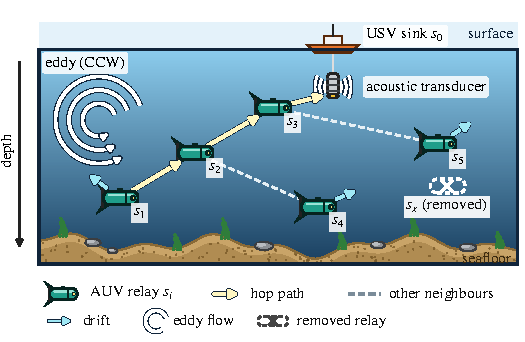
\includegraphics[width=\columnwidth]{fig1_network}

\caption{Network model (side view). Relays drift under an eddy and Gauss--Markov flow, so decodable links form and break; packets are forwarded hop by hop to the fixed sink. A relay that leaves the volume is removed. Each relay forwards using \emph{held} records of its neighbours, whose upkeep is the subject of this work.}
\label{fig:network}
\end{figure}

\subsection{Channel, Frames, and Energy}
\label{sec:channel}
Only the medium evaluates propagation and reception. The signal-to-noise ratio of a frame sent over a distance $d$ is
\begin{equation}
\mathrm{SNR}(d)=\mathrm{SL}-10\kappa\log_{10}d-\alpha(f_c)\,d-N_0,
\label{eq:snr}
\end{equation}
with source level $\mathrm{SL}$, spreading exponent $\kappa$, Thorp absorption $\alpha(f_c)$ at carrier frequency $f_c$, and ambient noise level $N_0$, all in decibels. Frames use non-coherent binary frequency-shift keying, for which the bit error rate is $p_b=\tfrac12\exp(-\gamma_b/2)$ with $\gamma_b=\mathrm{SINR}\cdot B/R_b$, and the frame error rate is $1-(1-p_b)^{\ell_f}$ for a frame of $\ell_f$ bits. Concurrent frames interfere, and a half-duplex node cannot receive while it transmits. A frame of $\ell_f$ bits occupies the channel for
\begin{equation}
T_f=T_{\mathrm{pre}}+\ell_f/R_b,
\label{eq:duration}
\end{equation}
so a short control frame is dominated by its preamble $T_{\mathrm{pre}}$. A node draws the powers $P_{\mathrm{tx}}$, $P_{\mathrm{rx}}$, and $P_{\mathrm{idle}}$ in the transmit, receive, and idle-listening states, and it listens continuously. A control frame therefore costs $T_f(P_{\mathrm{tx}}-P_{\mathrm{idle}})$ at the sender and $T_f(P_{\mathrm{rx}}-P_{\mathrm{idle}})$ at each receiver above the idle baseline, and it also consumes airtime that data frames could use.

\subsection{Locally Available Information}
\label{sec:info}
A node $s_i$ learns of a neighbour $s_j$ only by decoding a frame from it. Let $b_{ij}(t)$ be the latest time at which $s_i$ accepted a state-bearing frame from $s_j$, with $b_{ij}=-\infty$ if none. A record is \emph{fresh} when
\begin{equation}
L_{ij}(t)=\mathbf{1}\{b_{ij}(t)>-\infty,\; t-b_{ij}(t)\le T_{\mathrm{nb}}\},
\label{eq:fresh}
\end{equation}
and only fresh records can form candidates. At time $t$, the routing logic and the HELLO policy of $s_i$ may use only: its own state and timers; the fields of frames it has decoded, as written by the sender at transmission start; the received SNR and decode time of those frames; held records built from them, possibly stale; a-priori constants such as the PHY and MAC settings and the fixed sink position; and the outcome of its own transmissions. A node never reads another node's true position, depth, energy, or neighbour set.

\subsection{State Carriers and Host Interface}
\label{sec:carriers}
Each node $s_j$ has an advertised attribute vector $\xi_j(t)$ that its neighbours need, such as a value estimate, residual energy, depth or position, and a void flag. A frame carries a subset of it. We distinguish two \emph{state carriers} (Fig.~\ref{fig:carriers}). In the \emph{header-carried} regime, data frames carry the attributes, so a forwarding node advertises itself at no extra control cost, and a HELLO supplements this for nodes off the forwarding paths. In the \emph{HELLO-only} regime, data frames carry none, and a held record is written only by HELLO or beacon frames. Real protocols may mix the two. In Section~\ref{sec:eval}, the HELLO-only regime is a constructed variant of each host, not a reproduction of a published protocol.

\begin{figure}[t]
\centering
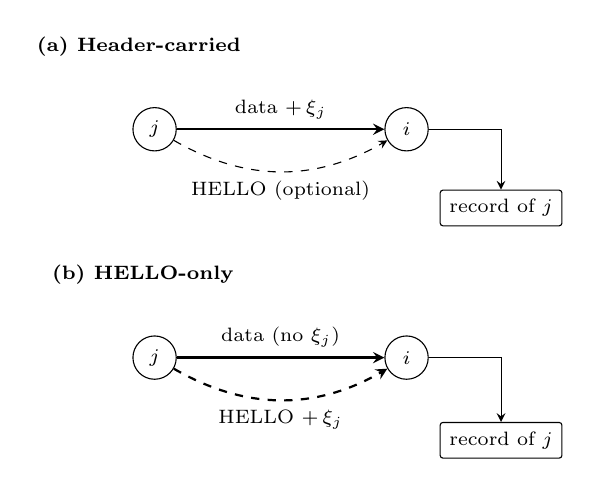
\begin{tikzpicture}[font=\scriptsize,>=stealth,node distance=0.5cm,
 nd/.style={circle,draw,minimum size=0.55cm,inner sep=0pt},
 tb/.style={draw,rounded corners=1pt,minimum width=1.5cm,minimum height=0.45cm,align=center}]
% panel a
\node[font=\scriptsize\bfseries] at (-0.2,2.55) {(a) Header-carried};
\node[nd] (a1) at (0,1.5) {$j$};
\node[nd] (a2) at (3.2,1.5) {$i$};
\draw[->,thick] (a1) -- node[above,pos=.5]{data $+\,\xi_j$} (a2);
\draw[->,dashed] (a1) to[bend right=30] node[below,pos=.5]{HELLO (optional)} (a2);
\node[tb] (ta) at (4.4,0.5) {record of $j$};
\draw[->] (a2) -| (ta);
% panel b
\node[font=\scriptsize\bfseries] at (-0.15,-0.35) {(b) HELLO-only};
\node[nd] (b1) at (0,-1.4) {$j$};
\node[nd] (b2) at (3.2,-1.4) {$i$};
\draw[->,thick] (b1) -- node[above,pos=.5]{data (no $\xi_j$)} (b2);
\draw[->,dashed,thick] (b1) to[bend right=30] node[below]{HELLO $+\,\xi_j$} (b2);
\node[tb] (tb) at (4.4,-2.45) {record of $j$};
\draw[->] (b2) -| (tb);
\end{tikzpicture}

\caption{The two state carriers. (a) Header-carried: a data frame writes the sender's attributes into the receiver's held record; a HELLO is optional. (b) HELLO-only: data frames write nothing, and a record exists only after a HELLO or beacon has been decoded, so maintenance determines whether a neighbour can be ranked at all.}
\label{fig:carriers}
\end{figure}

A host router $h$ is described by an eligible candidate set $\mathcal{I}^h_i(t)$ of node $s_i$, built from fresh records, and a forwarding output $\mathcal{R}_h$ that orders the candidates by a score $\sigma_i(j)$ and selects a next hop. The scheduler of Section~\ref{sec:design} uses the host through three primitives only: the candidate set and held records of the node itself, its own advertised vector, and a broadcast of a control frame. It does not use the host's learning rule. The hosts differ in their eligibility rules: in MARV a candidate has a fresh record, a held depth shallower than the sender, and no excluding void flag, and candidates are ordered by updated Q values; in QELAR a candidate has a fresh record and passes an admission test on its held SNR, without a depth restriction, and the largest stored Q value selects the next hop.

\subsection{Held State and Its Staleness}
\label{sec:stale}
Between two accepted frames from $s_j$, node $s_i$ holds a zero-order copy $\hat{\xi}_{ij}$ of the advertised vector, while the true attributes $\xi_j(t)$ keep evolving with motion, energy use, and learning. The copy is wrong for $s_i$'s purposes only if the error changes what $s_i$ does: whether $s_j$ is a candidate, how it ranks against another candidate, or whether $s_i$ can see $s_j$ at all. A record that is merely old is not necessarily wrong. This distinction, which Section~\ref{sec:problem} formalises, is what separates deciding when to re-advertise from running a timer.

\subsection{Metrics and Accounting}
\label{sec:metrics}
For a run $r$, let $G_r$ be the number of application packets generated in the analysis interval $[t_w,t_g)$ after a warm-up $t_w$, and $D_r$ the number of those packets that reach the sink. The run-level delivery ratio and energy per delivered bit are
\begin{equation}
p_r=\frac{D_r}{G_r},\qquad e_r=\frac{E_r}{\ell\,D_r},
\label{eq:runmetrics}
\end{equation}
where $\ell$ is the data payload length and $E_r$ is the modem energy of all nodes accumulated over $[t_w,t_g+t_d]$, which includes a drain period $t_d$ after the last generation. It covers transmit, receive, and idle-listening states, so idle energy is always counted, and it excludes propulsion and other platform loads. A relay that is removed stops generating packets, but packets it already offered stay in $G_r$. The packet cohort and the energy interval are therefore different intervals, and we do not call either of them ``the window''.

The primary summaries average run-level ratios, $\bar p=\mathbb{E}[p_r]$ and $\bar e=\mathbb{E}[e_r]$, over seeds. They differ from pooled estimates,
\begin{equation}
\hat p_{\mathrm{pool}}=\frac{\sum_r D_r}{\sum_r G_r},\qquad \hat e_{\mathrm{pool}}=\frac{\sum_r E_r}{\ell\sum_r D_r},
\label{eq:pooled}
\end{equation}
and one cannot be reported as the other. When $D_r=0$, $e_r$ is undefined, not zero, and the run's energy still belongs in the pooled numerator. The control overhead is
\begin{equation}
O_{\mathrm{ctrl}}=\frac{1}{t_g}\sum_{f\in\mathcal{F}}\frac{\ell_f}{8},
\label{eq:octrl}
\end{equation}
where $\mathcal{F}$ is the set of HELLO and beacon frames that start in $[0,t_g]$, with $\ell_f$ in bits. It charges the initial announcements and the sink beacon and excludes frames that start during the drain. The control count, the packet cohort, and the energy interval have deliberately different definitions.
